\documentclass[letterpaper,12pt]{article}
\usepackage{amsmath}
\usepackage{float}
\usepackage[margin=1in]{geometry}
\usepackage{graphicx}
\usepackage{placeins}
\usepackage{siunitx}
\usepackage[title]{appendix}
\usepackage{pdflscape}
\usepackage{tabularx}
\usepackage{times}
\usepackage{url}
\usepackage{setspace}
\usepackage[none]{hyphenat}

\DeclareSIUnit{\samplepersec}{SPS}

\begin{document}

\begin{titlepage}
    \begin{center}
        \vspace*{1cm}

        \Large
        \textbf{ELEC 490/498 Project Blueprint Document}

        \vspace{0.5cm}
        Group 18\\
        TeachEE\\
        \vspace{0.5cm}
        \normalsize
        \textbf{John Giorshev (20103586, john.giorshev@queensu.ca) \\ Eric Yang (20120750, e.yang@queensu.ca) \\ Ethan Peterson (20105011, 17emp5@queensu.ca) \\ Timothy Morland (20096286, 17tm22@queensu.ca)}\\
        \vspace{0.5cm}
        Submitted November 22, 2022\\

        \vfill
            
        \textbf{To:}\\
        Instructor and Supervisor Dr. Sean Whitehall (sw109@queensu.ca) \\
        Supervisor Dr. Thomas Dean (tom.dean@queensu.ca) \\
            
        \vspace{1.8cm}

    \end{center}
\end{titlepage}
\section*{Executive Summary}
% pop a one pager in here. Ideally less
% Timothy
\newpage

\tableofcontents
\listoffigures
\listoftables
\newpage
\setstretch{1.5}
\section{Introduction} \label{sec:intro} % John
% As short as possible. Total BS LMAO
Welcome to this 1.5 spaced introduction. it should be 1.5 spaced. See the
setstretch command shown above in the tex file.

\subsection{Design Problem}
TeachEE is a device that acts as a general purpose electronics measurement
instrument for remotely delivered engineering labs. The device acts as both a
USB oscilloscope and current monitor. At a design level, the device will require
both a custom Printed Circuit Board, device driver, and graphical user interface
to function correctly. There are two key technical challenges in this project;
the Printed Circuit Board (PCB) and device driver software.
\\~\\
The PCB is a large technical undertaking as the PCB must be able to capture both
voltage and current samples at a rate that is useful to undergraduate student.
Moreover, the PCB must contain custom circuitry to relay the sample data over
USB. USB is a high speed interface requiring controlled impedance transmission
lines on the PCB. Additionally, the PCB will need multiple high speed clocks for
the USB PHY and Analog to Digital Converter (ADC). There are also further
technical challenges with respect to the analog signalling and sufficiently
filtering and protecting the inputs.
\\~\\
The second key technical challenge in this project is the device driver for the
oscilloscope. The USB 2.0 link between the device and laptop has a throughput as
high as 480 Mbps. This requires performant driver software that can process the
sample data in a timely manner and relay it to the GUI frontend. In addition to
the requirement for low latency, the software will also require a packet framing
technique that can efficiently separate current and voltage samples.
% Ethan
% Explain the design problem Hardware software timeline
% 275 words max
\subsection{System Specifications}
Since the TeachEE has both a hardware and software component. The system
specifications have been broken up into hardware and software tables
respectively.

% \newcolumntype{b}{X}
% \newcolumntype{s}{>{\hsize=.2\hsize}X}
% \newcolumntype{m}{>{\hsize=.4\hsize}X}
\begin{table}[h!]
    \caption{Hardware Specifications}
    \begin{tabularx}{\textwidth}{l|l|l|l}
          & Specification & Target Value & Tolerance \\
        \hline
        1 &Voltage Input Bandwidth&\SI{100}{\kilo\hertz}& $\pm \SI{1}{\kilo\hertz}$ \\
        2 &Current Input Bandwidth&\SI{100}{\kilo\hertz}& $\pm \SI{1}{\kilo\hertz}$ \\
        3 &Measureable Current Range&\SI{-15}{\ampere} to \SI{+15}{\ampere}& $\pm \SI{5}{\ampere}$ \\
        4 &Measureable Voltage Range&\SI{0}{\volt} to \SI{3.3}{\volt}& $\pm \SI{200}{\milli\volt}$ \\
        5 &Number of Current Input Channels& $1$ & $0$ \\ 
        6 &Number of Voltage Input Channels& $1$ & $+2$ \\
        7 &Power Input Voltage Rating& \SI{5}{\volt} & $\pm \SI{500}{\milli\volt}$ \\
        8 &Power Current Consumption Rating& \SI{500}{\milli\ampere} & $\pm \SI{250}{\milli\ampere}$ \\
        9 &Voltage Sample Rate& \SI{1}{\mega\samplepersec} & \SI{0}{\mega\samplepersec}\\
        10 &Current Sample Rate& \SI{1}{\mega\samplepersec} & \SI{0}{\mega\samplepersec} \\
        11 &PCB Thickness& \SI{1.6}{\milli\metre} & $\pm \SI{0.1}{\milli\metre}$ \\
        12 &PCB Dimensions& \SI{0.04}{\meter\squared} & $\pm \SI{400}{\milli\metre\squared}$
    \end{tabularx} 
\label{hw:specs-table}
\end{table}

% Timbo / Ethan
\begin{table}[h!]
    \caption{Software Specifications}
    \begin{tabularx}{\textwidth}{l|l}
        \textbf{1} & \textbf{Functional Requirements}\\
        \hline
        1.1 & The software shall be able to modulate the sample rate. \\
        1.2 & The software shall be able to modify the trigger voltage. \\
        \hline
        \textbf{2} & \textbf{Interface Requirements} \\
        \hline
        2.1 & Something about driver interface to GUI Idk (write in the formal format I showed above plz) \\
        2.1 & Also try to write some stuff about how FTDI driver interfaces with backend which in turn interfaces with frontend. What are the interface signatures and tools used? \\
        \hline
        \textbf{3} & \textbf{Performance Requirements} \\
        \hline
        3.1 & The software shall be able to render waveforms at a rate of \SI{30}{\hertz} on screen.
    \end{tabularx} 
\label{hw:specs-table}
\end{table}


% 1-2 tables (maybe one for HW SW)
% Ethan will write some hardware and software specs here in a table

\section{Work Breakdown Structure} % ERIC
% 1.5 pages max for everything
\subsection{Approach} 
\subsection{Design Tools, Hardware, Instrumentation}
\subsection{Validation}

\section{Progress to Date} % Ethan / Tim for HW/SW respectively
Since TeachEE is a project originally proposed in ELEC390, there is progress in
the development of hardware and software.
% Explain that there has been a completed hardware design.
% include schematics, layout and BOM in Appendices

\subsection{Hardware Design}
As of this blueprint submission, the initial printed circuit board schematic and
layout are complete. The PCB system block diagram is shown in the figure below.
Full schematic and layout prints are supplied in Appendix
\ref{appendix:schematic} and \ref{appendix:layout} respectively.
\begin{figure}[h!]
    \centering
    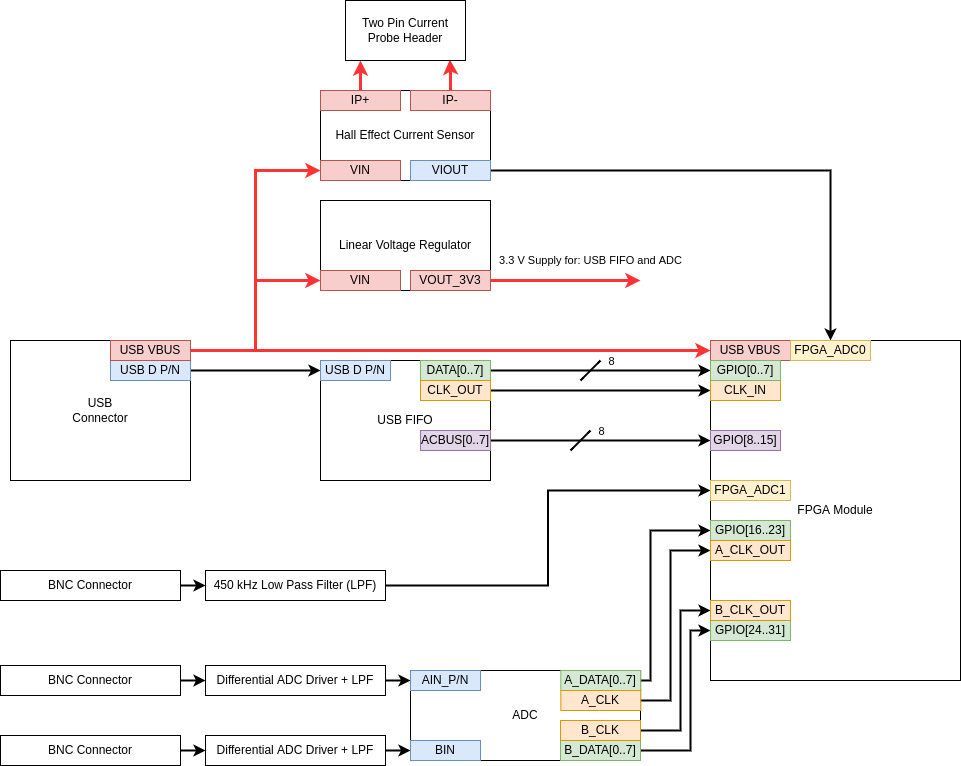
\includegraphics[width=16cm]{../../misc/TeachEE-System-Diagram.drawio.png}
    \caption{TeachEE PCB System Block Diagram}
    \label{fig:pcb-block-diagram}
\end{figure}
% Add note that you can find the full Bill of materials below.
% discuss the speed the FIFO will be capable of.
% Discuss the max sample rate of the ADC
% Discuss sampling theorem and LPFs / analog front end stuff.
% maybe also add references to datasheets of major components
\subsection{Software Design}
\subsection{Milestones and Division of Labour}
% Table of major and intermediate milestones (ERIC)
% Each table cell should include due date and assigned member
\section{Budget} % Ethan
% include some preamble wrt board quantities and BOM table
% consider ActiveBOM from Altium for this.
% BOM probably takes too many pages, will need to attenuate
\subsection{Materials and Supplies}
\subsection{Contributions From Other Sources}
% None for the time being. Will be in touch w supervisor for support if we order additional units

\section{Potential Problems and Mitigation Strategies}
% Ethan (Make a single table)
\section{Strategies to address the wider impact of the project}
% John 0.5 pages max also just some BS (maybe how it can change labs for the
% better as a business proposition)
\section{Conclusion}
% Tim (0.5 pages of BS is an order)
\newpage
% For this references section we need to at least reference our 390 report
\bibliographystyle{IEEEtran}
\bibliography{./report}
\newpage

\begin{appendices}
    \section{Schematics}
    \label{appendix:schematic}
    \section{PCB Layout}
    \label{appendix:layout}
    \section{Full Bill of Materials}
    \label{appendix:bom}
\end{appendices}
\end{document}